% ============================================================
%  M.Sc. in High-Performance Computing thesis presentation
%  Communication-Avoiding Krylov Exponential Integration
%  for Multi-GPU Option Pricing
%
%  Speaker    : Kevin Knights
%  Supervisor : Prof. Kirk M. Soodhalter
%  Trinity College Dublin, School of Mathematics
%
%  Structure: title, outline, four sections of 12 main slides,
%  then an appendix held in reserve for examiner questions.
% ============================================================

\documentclass{beamerTCD}

\usepackage{tcd-msc-hpc-presentation}
\usepackage{amsmath,amssymb}
\usepackage{booktabs,dcolumn}
\usepackage{graphicx}
\usepackage{inconsolata}
\usepackage{array}
\usetikzlibrary{positioning,arrows.meta,backgrounds,fit}

\urlstyle{tt}

\institute{MSc.\ High Performance Computing\\School of Mathematics, Trinity College Dublin}

\hypersetup{%
   pdfsubject  = {TCD M.Sc. in High-Performance Computing thesis presentation},
   pdftitle    = {Communication-Avoiding Krylov Exponential Integration
                  for Multi-GPU Option Pricing},
   pdfkeywords = {communication avoiding, Krylov subspace methods, exponential
                  integrator, matrix powers, s-step, CholeskyQR2, GPU, NCCL,
                  option pricing, Black-Scholes},
   pdfpagemode = FullScreen,
   colorlinks  = false,
   urlcolor    = TCDPurple,
}

\setbeamertemplate{navigation symbols}{}
\setbeamertemplate{headline}{}          % the theme's section bar is not wanted
\setbeamerfont{frametitle}{size=\large}

% Section dividers: one compact roadmap frame before each part, so the
% audience can always see which part of the argument is on screen.
\setbeamertemplate{section in toc}{%
  \inserttocsectionnumber.~\inserttocsection}
\AtBeginSection[]{%
  {\setbeamertemplate{footline}{}
  \begin{frame}[c]{}
    \vfill
    \begin{center}
      \begin{minipage}{0.82\textwidth}
        \tableofcontents[currentsection, sectionstyle=show/shaded]
      \end{minipage}
    \end{center}
    \vfill
  \end{frame}}}

\newcommand{\mat}[1]{\mathbf{#1}}
\newcommand{\vect}[1]{\mathbf{#1}}
\newcommand{\Rv}{R_v}
\newcommand{\Rh}{R_h}
\newcommand{\tred}{t_{\mathrm{red}}}
\newcommand{\tredstar}{t^{\star}_{\mathrm{red}}}
% marks a slide whose content is my own contribution
\newcommand{\mine}{{\color{TCDBlue}$\bigstar$}}

\title[When does communication avoidance pay?]{%
  Communication-Avoiding \\Krylov Exponential Integration\\
  for Multi-GPU Option Pricing}

\author[Knights K.]{%
  Kevin Knights
  \\\small Supervisor: Prof.\ Kirk M.\ Soodhalter}

\date{\today}

% ============================================================
\begin{document}
% ============================================================

  {\setbeamertemplate{footline}{}
  \begin{frame}
  \titlepage
  \vskip-2em
  \begin{figure}
      
\includegraphics[scale=.085]{Trinity_Main_Logo.jpg}
  \end{figure}
  \end{frame}
  }

% -----------------------------------------------------------
% OUTLINE  |  motivation and roadmap
% -----------------------------------------------------------
\begin{frame}[t]{What this talk argues}
\small

  A trading desk reprices the same multi-asset PDE across a whole book, so the
  cost of \emph{one} solve sets valuation throughput. That solve is dominated
  by \textbf{moving data}, not arithmetic, which is what
  \emph{communication-avoiding} methods target.

  \vskip0.3em
  \begin{alertblock}{}\footnotesize
    \centering
    The question is not \emph{how} to avoid communication, but
    \textbf{when it is worth doing.}
  \end{alertblock}

  \vskip0.4em
  \begin{columns}[T]
    \column{0.60\textwidth}
    \begin{enumerate}\scriptsize
      \item \textbf{The problem and the method}\\
            the operator, and one exponential action per step
      \item \textbf{Where the time goes}\\
            profiling, the two CA mechanisms, and a null result
      \item \mine\ \textbf{The regime map}\\
            two a-priori coordinates that predict the opportunity
      \item \mine\ \textbf{Does it pay?}\\
            a distributed CA integrator on four GPUs
    \end{enumerate}

    \column{0.38\textwidth}\footnotesize
    \begin{block}{\footnotesize Method in one line}\footnotesize
      Predict the opportunity \emph{before} building the kernel, then measure
      whether the prediction holds.
    \end{block}
    \vskip0.2em
    \centerline{\scriptsize \mine\ marks my own contribution.}
  \end{columns}

\end{frame}

% ===========================================================================
\section{The problem and the method}
% ===========================================================================

% -----------------------------------------------------------
% SLIDE 1  |  The operator
% -----------------------------------------------------------
\begin{frame}[t]{The problem: one operator, solved over and over}
\small

  Three-asset Black--Scholes in log prices, backward in $\tau = T-t$, for a
  \textbf{basket call} and a \textbf{rainbow min-call}:
  \vskip-0.2em
  \[
    \frac{\partial u}{\partial \tau}
      = \underbrace{\tfrac{1}{2}\!\sum_{d,d'}\!\rho_{dd'}\sigma_d\sigma_{d'}
        \frac{\partial^2 u}{\partial x_d \partial x_{d'}}}_{\text{diffusion}+\text{correlation}}
      + \underbrace{\sum_d\!\left(r-\tfrac{1}{2}\sigma_d^2\right)\!
        \frac{\partial u}{\partial x_d}}_{\text{convection}}
      \underbrace{-\,r u}_{\text{reaction}} + \;b(\tau)
  \]

  \medskip
  Second-order central differences on a uniform grid, $N=n^3$ unknowns:
  \begin{itemize}
    \item $\mat A$ carries \textbf{19 nonzeros per row} and $O(N_1N_2)$
          bandwidth, which rules out banded direct solvers at scale.
    \item Convection is skew-symmetric, so $\mat A$ is
          \textbf{non-symmetric and non-normal}.
    \item Stiffness grows as $\|\mat A\|\sim O(n^2)$.
  \end{itemize}

  \vskip0.5em
  \begin{exampleblock}{}\footnotesize
    \centering
    Production resolution is $n=61$: \textbf{226{,}981 unknowns},
    4.23\,M nonzeros.
  \end{exampleblock}

\end{frame}

% -----------------------------------------------------------
% SLIDE 2  |  The method
% -----------------------------------------------------------
\begin{frame}[t]{The method: one exponential action per time step}
\small

  \vskip0.2em
  Discretizing space only leaves time continuous: the PDE becomes a large
  linear system of ODEs, one equation per grid point.
  \vskip0.1em
  \[
    \frac{d\vect u}{d\tau} = \mat A\vect u + \mat B\vect s(\tau),
    \qquad \vect u(0)=\vect u_0 \quad(\text{the payoff}).
  \]

  \vskip0.5em
  The basket's boundary forcing is polynomial, $\vect s'=\mat K\vect s$ with
  $\mat K$ nilpotent, so it is absorbed \emph{exactly} into an autonomous
  augmented system:
  \vskip0.1em
  \[
    \widetilde{\mat A}=\begin{bmatrix}\mat A&\mat B\\ \mat 0&\mat K\end{bmatrix},
    \qquad
    \boxed{\;\widetilde{\vect v}=\begin{bmatrix}\vect u_k\\ \vect s(\tau_k)\end{bmatrix},
    \qquad M=N+3\;}
  \]

  \vskip0.6em
  One time step is then \emph{one matrix-exponential action}, approximated in
  the Krylov subspace $\mathcal K_m(\mat G,\widetilde{\vect v})$ with
  $\mat G = h\widetilde{\mat A}$:
  \vskip0.1em
  \[
    \vect u_{k+1}=e^{\mat G}\widetilde{\vect v}
    \;\approx\;
    \beta\,\mat V_m\, e^{\mat H_m}\vect e_1 ,
    \qquad \beta=\|\widetilde{\vect v}\| .
  \]

  \vskip0.5em
  \centerline{\footnotesize Arnoldi on $\mat G$ builds $\mat V_m$ and
              $\overline{\mat H}_m$; $m$ grows adaptively until the endpoint
              defect $\eta_m<10^{-8}$.}

\end{frame}

% ===========================================================================
\section{Where the time goes}
% ===========================================================================

% -----------------------------------------------------------
% SLIDE 3  |  Profiling
% -----------------------------------------------------------
\begin{frame}[t]{Profiling: two kernels, two different ceilings}
\small

  \vskip-0.2em
  \begin{columns}[c]
    \column{0.45\textwidth}
    \begin{center}\footnotesize
    \begin{tabular}{@{}lcc@{}}\toprule
      \textbf{Kernel} & $n{=}31$ & $n{=}61$ \\\midrule
      SpMV                   & 83.5\% & 78.0\% \\
      MGS                    & 11.4\% & 16.6\% \\
      dense $\exp(\mat H_m)$ & 0.40\% & 0.23\% \\\midrule
      mean $m$               & 7.60   & 8.91   \\\bottomrule
    \end{tabular}
    \end{center}
    \vskip-0.2em
    \centerline{\scriptsize share of KSM-EI solve time}
    \vskip0.8em
    \footnotesize
    Grids follow Niesen \& Wright's option-pricing study, so the semi-discrete
    ODE error stays comparable with theirs.

    \column{0.53\textwidth}
    \vskip-0.6em
    \begin{figure}
      \centering
      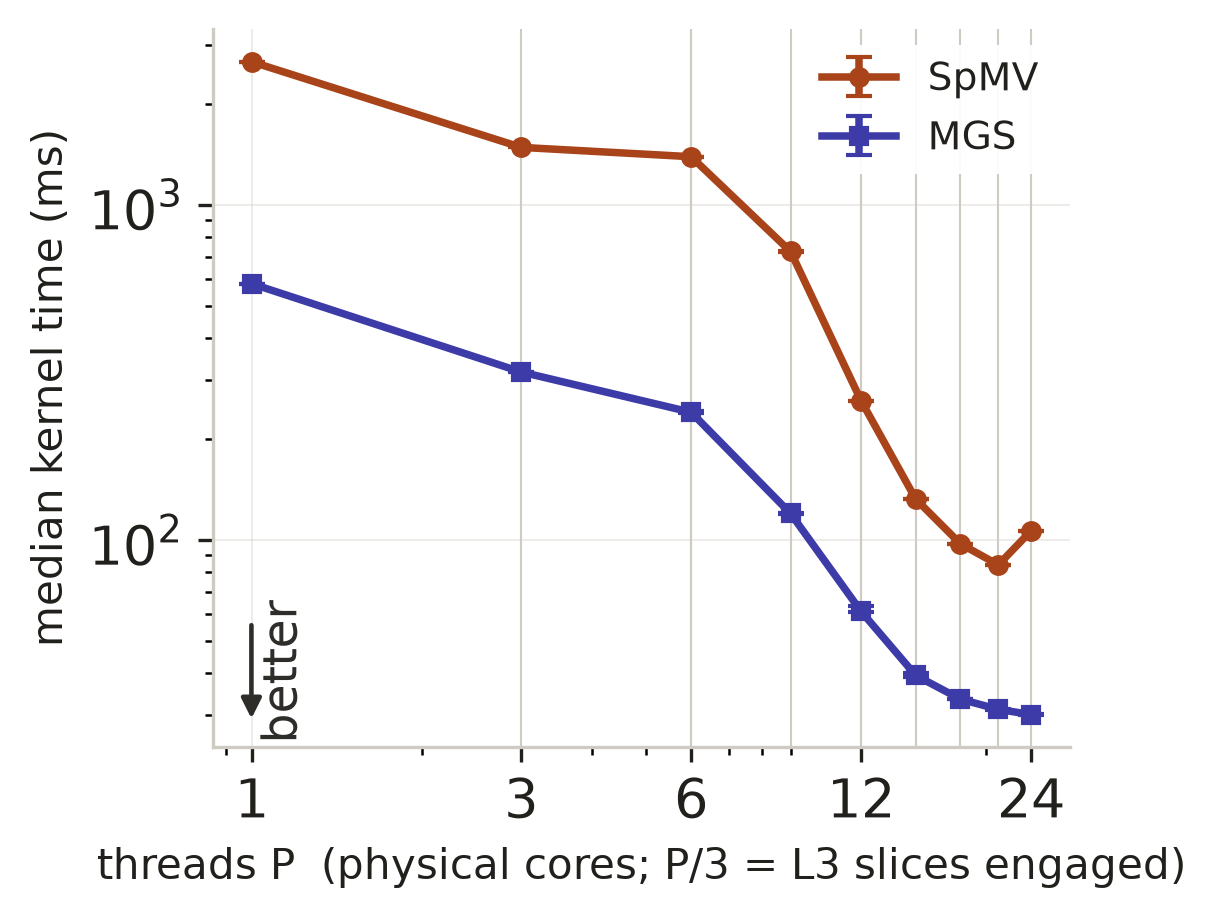
\includegraphics[width=0.99\linewidth]{pres_scaling_strong.png}
    \end{figure}
    \vskip-1.1em
    \centerline{\scriptsize Strong scaling at $n{=}61$: fixed work, more cores.}
  \end{columns}

  \vskip0.6em
  \begin{exampleblock}{}\footnotesize
    \centering
    SpMV plateaus until the working set fits the engaged cache. Modified
    Gram--Schmidt (MGS) keeps improving, but every inner product it performs
    is a global reduction, and its share grows with $m$.
  \end{exampleblock}

\end{frame}

% -----------------------------------------------------------
% SLIDE 4  |  Communication avoidance
% -----------------------------------------------------------
\begin{frame}[t]{Communication avoidance: two mechanisms}
\small

  \textbf{The obstacle.} Arnoldi iteration $j$ needs $\vect v_j$ before it can
  start: one SpMV and one global reduction per step, strictly in sequence.

  \vskip0.5em
  \textbf{1. One deep exchange, not $q-1$.}
  \vskip0.1em
  \begin{center}
  \scalebox{0.60}{%
  \begin{tikzpicture}[
    lbl/.style={font=\scriptsize,text=TCD-Grey},
    ghost/.style={draw=TCD-Grey-ii,fill=TCD-Grey-iii},
    msg/.style={-{Latex[length=5pt]},TCD-Red,thick}]
    \fill[TCDBlue] (0,0) rectangle (2.8,1.2);
    \node[white,font=\scriptsize\bfseries] at (1.4,0.6) {owned slab};
    \foreach \k in {0,1,2}{
      \draw[ghost] (0,1.25+\k*0.30) rectangle (2.8,1.51+\k*0.30);
      \draw[msg] (3.15,1.38+\k*0.30) -- (2.95,1.38+\k*0.30);
    }
    \node[lbl,anchor=west] at (3.25,1.78) {$q-1$ messages};

    \begin{scope}[xshift=7.4cm]
      \fill[TCDBlue] (0,0) rectangle (2.8,1.2);
      \node[white,font=\scriptsize\bfseries] at (1.4,0.6) {owned slab};
      \draw[ghost] (0,1.25) rectangle (2.8,2.11);
      \node[lbl] at (1.4,1.68) {$q-1$ planes};
      \draw[msg,line width=1.6pt] (3.35,1.68) -- (2.95,1.68);
      \node[lbl,anchor=west] at (3.45,1.68) {\textbf{1} message, same bytes};
    \end{scope}
  \end{tikzpicture}}
  \end{center}

  \vskip0.5em
  \textbf{2. One block, not $m$ vectors.} Orthogonalize a whole Krylov block at
  once with \textbf{CholeskyQR2}: form the Gram matrix
  $\mat Z^{\mathsf T}\mat Z$, Cholesky-factor it, repeat once for stability.
  \vskip-0.2em
  \[
    \mat Z_q=[\vect v,\ \mat A\vect v,\ \ldots,\ \mat A^{q-1}\vect v]
    \qquad
    \underbrace{1+\tfrac{m(m+3)}{2}}_{\text{MGS}}
    \;\longrightarrow\;
    \underbrace{1+2\lceil m/q\rceil}_{\text{one block}}
  \]

  \vskip0.2em
  \begin{exampleblock}{}\footnotesize
    \centering
    Messages fall from $q-1$ to one and reductions by \textbf{11--16$\times$}
    at the measured $m=8$--$11$, $q=8$; the price is recomputing the ghost
    region.
  \end{exampleblock}

\end{frame}

% -----------------------------------------------------------
% SLIDE 5  |  On puffin it does not pay
% -----------------------------------------------------------
\begin{frame}[t]{On puffin it does not pay}
\small

  Both mechanisms built and timed on \emph{puffin}, a 24-core Threadripper
  3960X on a single NUMA socket.

  \vskip0.2em
  \begin{columns}[T]
    \column{0.49\textwidth}
    \vskip-0.6em
    \begin{figure}
      \centering
      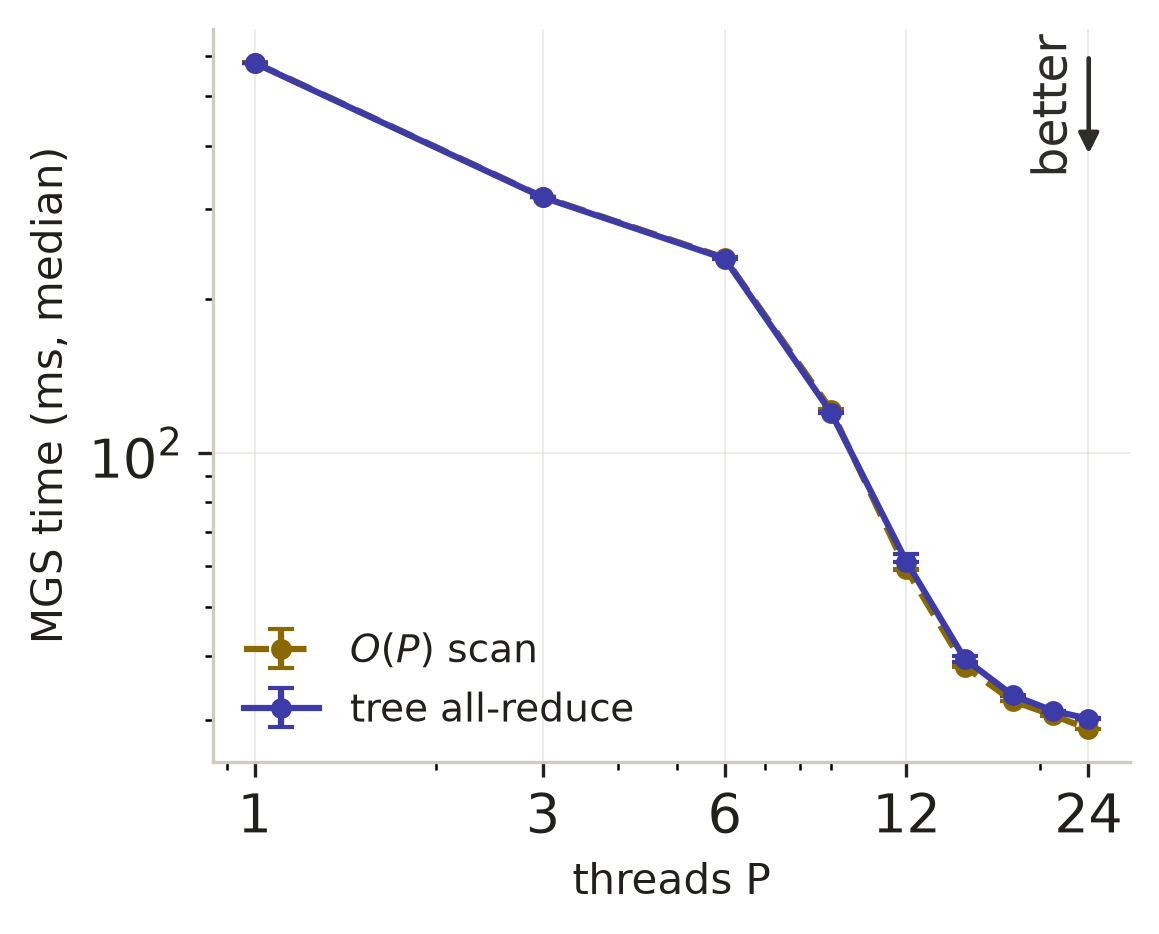
\includegraphics[width=\linewidth]{pres_scaling_reduction.png}
    \end{figure}
    \vskip-1.0em
    \centerline{\scriptsize \textbf{Horizontal:} a $1.7\times$ faster all-reduce}
    \centerline{\scriptsize leaves MGS within 5\%.}

    \column{0.49\textwidth}
    \vskip-0.6em
    \begin{figure}
      \centering
      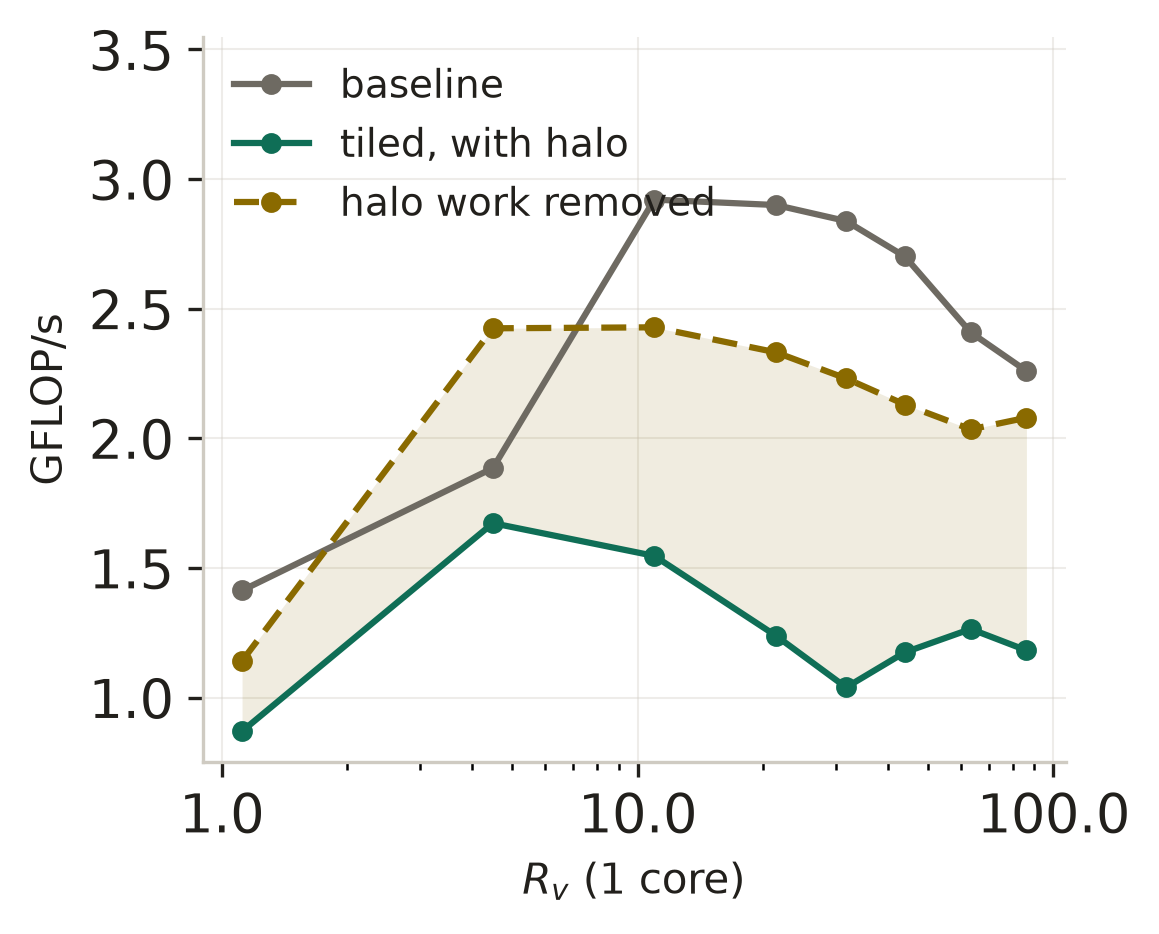
\includegraphics[width=\linewidth]{pres_sweep_mechanism.png}
    \end{figure}
    \vskip-1.0em
    \centerline{\scriptsize \textbf{Vertical (L2):} the gap is the halo.}
    \centerline{\scriptsize The L3 sweep agrees.}
  \end{columns}

  \vskip0.4em
  \begin{alertblock}{}\footnotesize
    \centering
    $11$--$16\times$ fewer reductions, $4$--$8\times$ less modeled traffic.\\
    \textbf{The saving is real; the speedup is not. So when \emph{does} it pay?}
  \end{alertblock}

\end{frame}

% ===========================================================================
\section{The regime map}
% ===========================================================================

% -----------------------------------------------------------
% SLIDE 6  |  The regime map
% -----------------------------------------------------------
\begin{frame}[t]{The regime map: predict first, then measure}
\small

  \vskip-0.2em
  \centerline{$\displaystyle
    \Rv=\frac{\text{Arnoldi working set}}{\text{last-level cache}}
    \qquad\qquad
    \Rh=\frac{\text{reduction latency}}{\text{compute between reductions}}$}

  \vskip-0.3em
  \begin{figure}
    \centering
    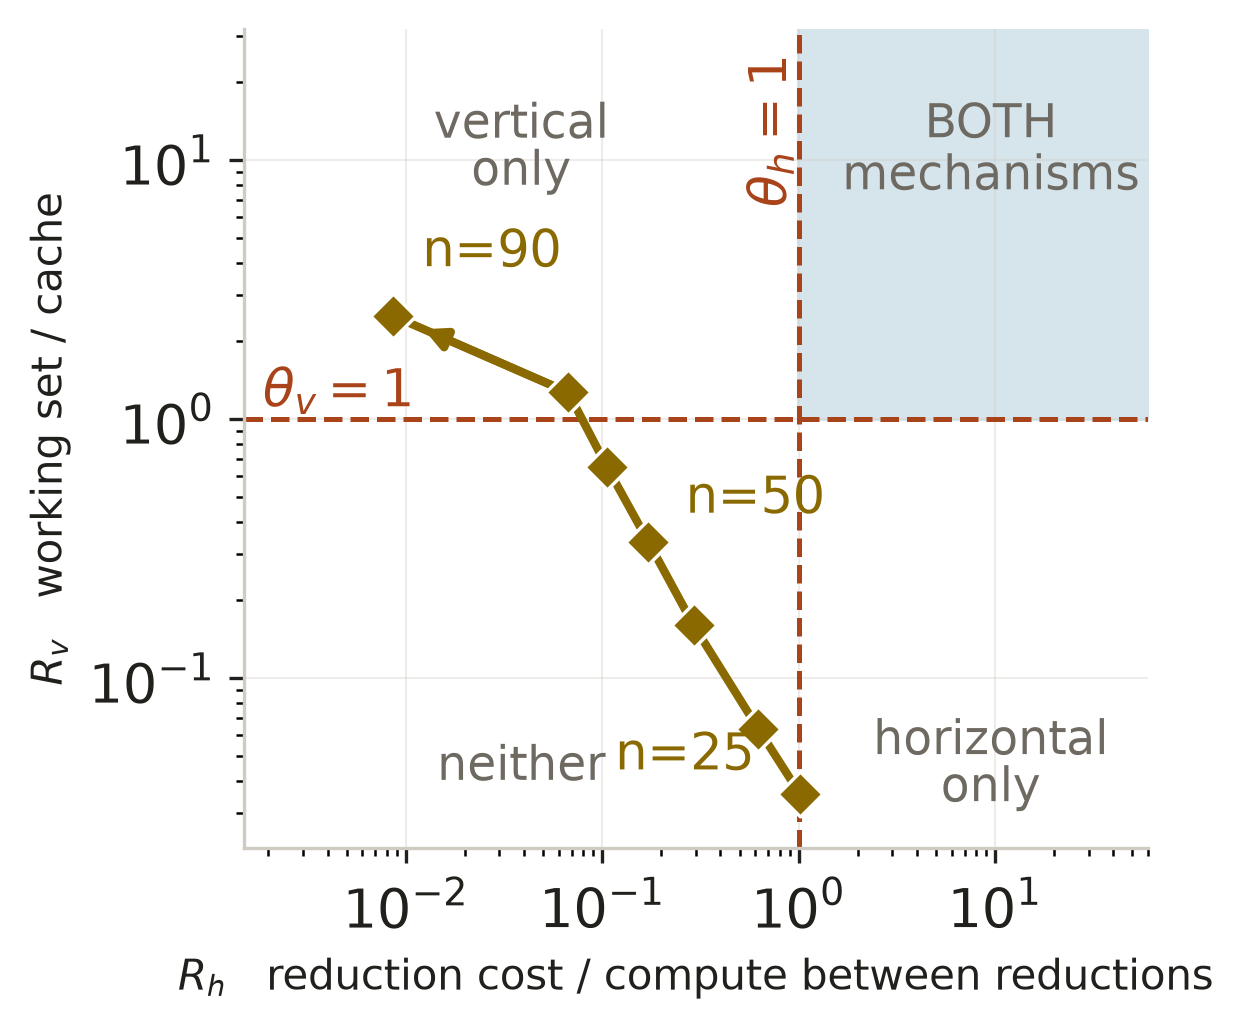
\includegraphics[height=0.585\textheight]{regime_trajectory_puffin.png}
  \end{figure}
  \vskip-0.9em
  \centerline{\scriptsize Eight production grids, $n=25\to90$, real basket
              operator, puffin's calibrated constants.}

  \vskip0.3em
  \begin{exampleblock}{}\footnotesize
    \centering
    On one socket $\Rv\Rh$ stays near $0.04$ for every $P$, so the corner is
    not merely unreached here: it is unreachable on this topology.
  \end{exampleblock}

\end{frame}

% -----------------------------------------------------------
% SLIDE 7  |  How the coordinates are built
% -----------------------------------------------------------
\begin{frame}[t]{How the coordinates are built}
\small

  \vskip0.4em
  \textbf{$\Rv$, from the problem.} Working-set bytes implied by $N$, the
  sparsity pattern and the measured Krylov dimension $m$, over the last-level
  cache actually available to the team:
  \vskip0.1em
  \[
    \Rv = \frac{\text{bytes}(N,\ \mathrm{nnz},\ m)}{C_{\text{LLC}}(P)} .
  \]

  \vskip0.6em
  \textbf{$\Rh$, from a calibration instrument.} An isolated scalar all-reduce
  with no application work, fitted over the tree levels it crosses:
  \vskip0.1em
  \[
    \Rh = \frac{\tred(P)}{W_{\text{local}}} ,
    \qquad
    \tred(P) = t_{\text{intra}}L_{\text{in}}
             + t_{\text{cross}}\min(L_{\text{x}},L^{\star}) .
  \]

  \vskip0.8em
  \begin{alertblock}{}\footnotesize
    \centering
    \textbf{Raising the cost of a reduction is what moves an operator right,
    and that is a property of topology.} \\Puffin tops out at
    $\tred = 1.70\,\mu$s, and the corner opens at about $25\,\tred$.
  \end{alertblock}

\end{frame}

% -----------------------------------------------------------
% SLIDE 8  |  The GPU regime map
% -----------------------------------------------------------
\begin{frame}[t]{More participants push the operator into the corner}
\small

  \vskip0.3em
  \begin{columns}[c]
    \column{0.56\textwidth}
    \begin{figure}
      \centering
      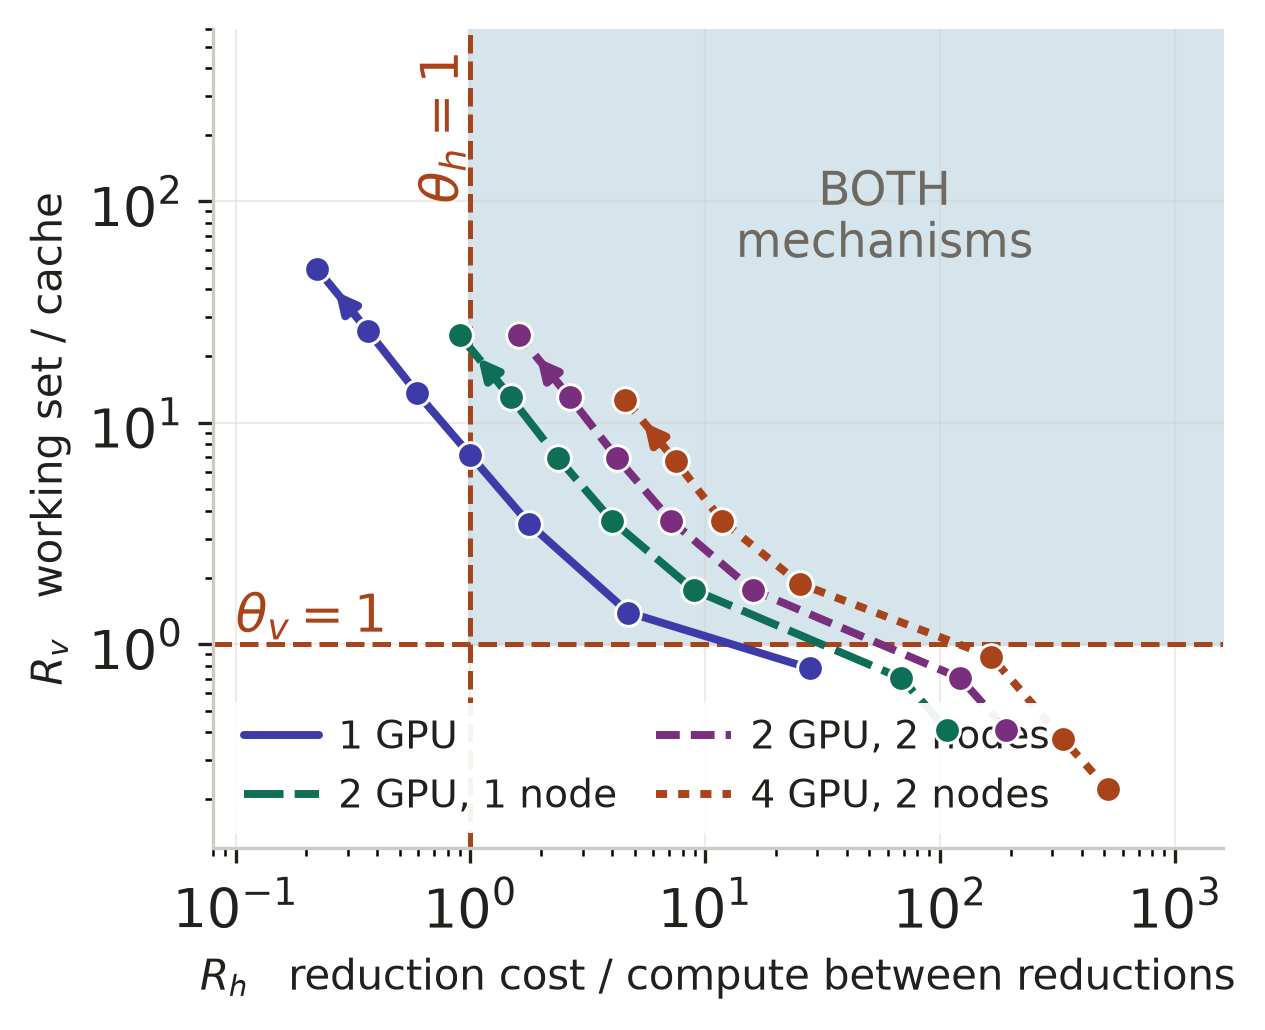
\includegraphics[width=\linewidth]{regime_trajectory_synge_grid.png}
    \end{figure}

    \column{0.42\textwidth}\footnotesize
    Same definitions, recalibrated machine constants. Synge is two nodes with
    two Tesla V100s each.

    \smallskip
    A GPU crosses \textbf{five} reduction levels where the CPU crosses two, and
    every added participant raises $\tred$, moving the whole trajectory
    \textbf{right}.

    \smallskip
    At $n{=}61$, $m{=}12$, $q{=}8$ the coordinates are
    $\Rv=7.2$ and $\Rh=1.7$: inside the corner on both cards.
  \end{columns}

  \vskip0.2em
  \centerline{\scriptsize Each line sweeps the same grids: $n{=}25$ at the lower
              right to $n{=}90$ at the upper left.}

\end{frame}

% ===========================================================================
\section{Does it pay?}
% ===========================================================================

% -----------------------------------------------------------
% SLIDE 9  |  The roofline gate
% -----------------------------------------------------------
\begin{frame}[t]{Reaching the corner is not enough: the device's roofline}
\small

  \vskip0.2em
  \begin{columns}[c]
    \column{0.56\textwidth}
    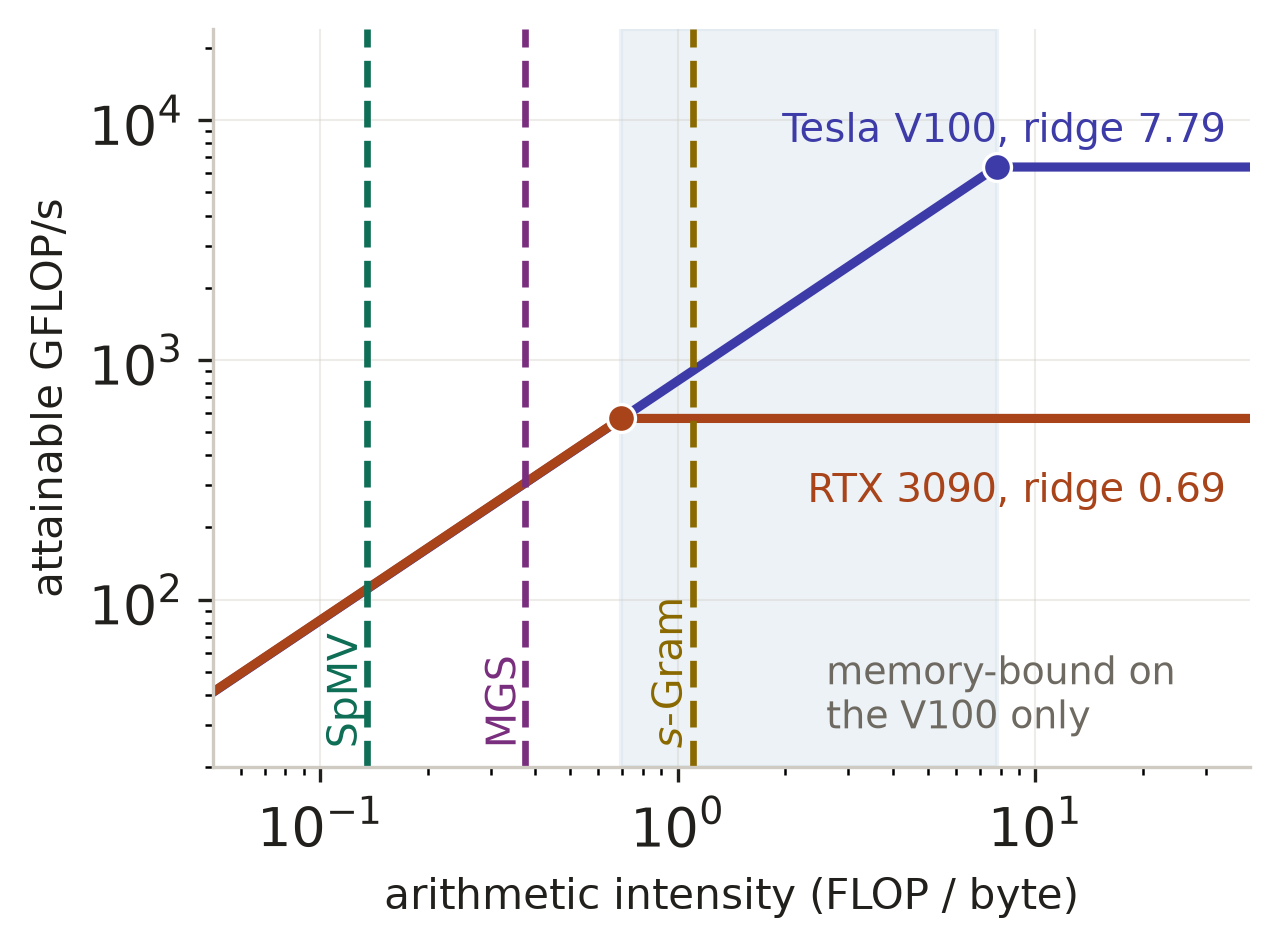
\includegraphics[width=0.96\linewidth]{pres_gpu_gate.png}

    \column{0.42\textwidth}
    \centerline{\scriptsize\textbf{Nsight Compute, $s$-Gram kernel}}
    \vskip0.2em
    \begin{center}\scriptsize\setlength{\tabcolsep}{4pt}
    \begin{tabular}{@{}lcc@{}}\toprule
      \textbf{\% of roof} & \textbf{V100} & \textbf{3090} \\\midrule
      DRAM    & \textbf{86\%} & 38\% \\
      compute & 16\%          & \textbf{94\%} \\\midrule
      verdict & memory        & compute \\
      \bottomrule
    \end{tabular}
    \end{center}
  \end{columns}

  \vskip0.6em
  \begin{block}{\footnotesize The memory-bound check}\footnotesize
    A precondition, before the map is read: compare each kernel's arithmetic
    intensity ($AI$, FLOP per byte) with the FP64 ridge, peak FP64 over
    achieved bandwidth ($BW$).
    \vskip-0.4em
    \[
      AI_{\text{kernel}}
      \;<\;
      \underbrace{\frac{\text{peak FP64}}{BW_{\text{achieved}}}}_{\text{FP64 ridge}}
      \;\Longrightarrow\;
      \text{memory-bound, and on the map.}
    \]
  \end{block}

\end{frame}

% -----------------------------------------------------------
% SLIDE 10  |  The CA result
% -----------------------------------------------------------
\begin{frame}[t]{Does communication avoidance pay?}
\small

  \vskip-0.4em
  \begin{figure}
    \centering
    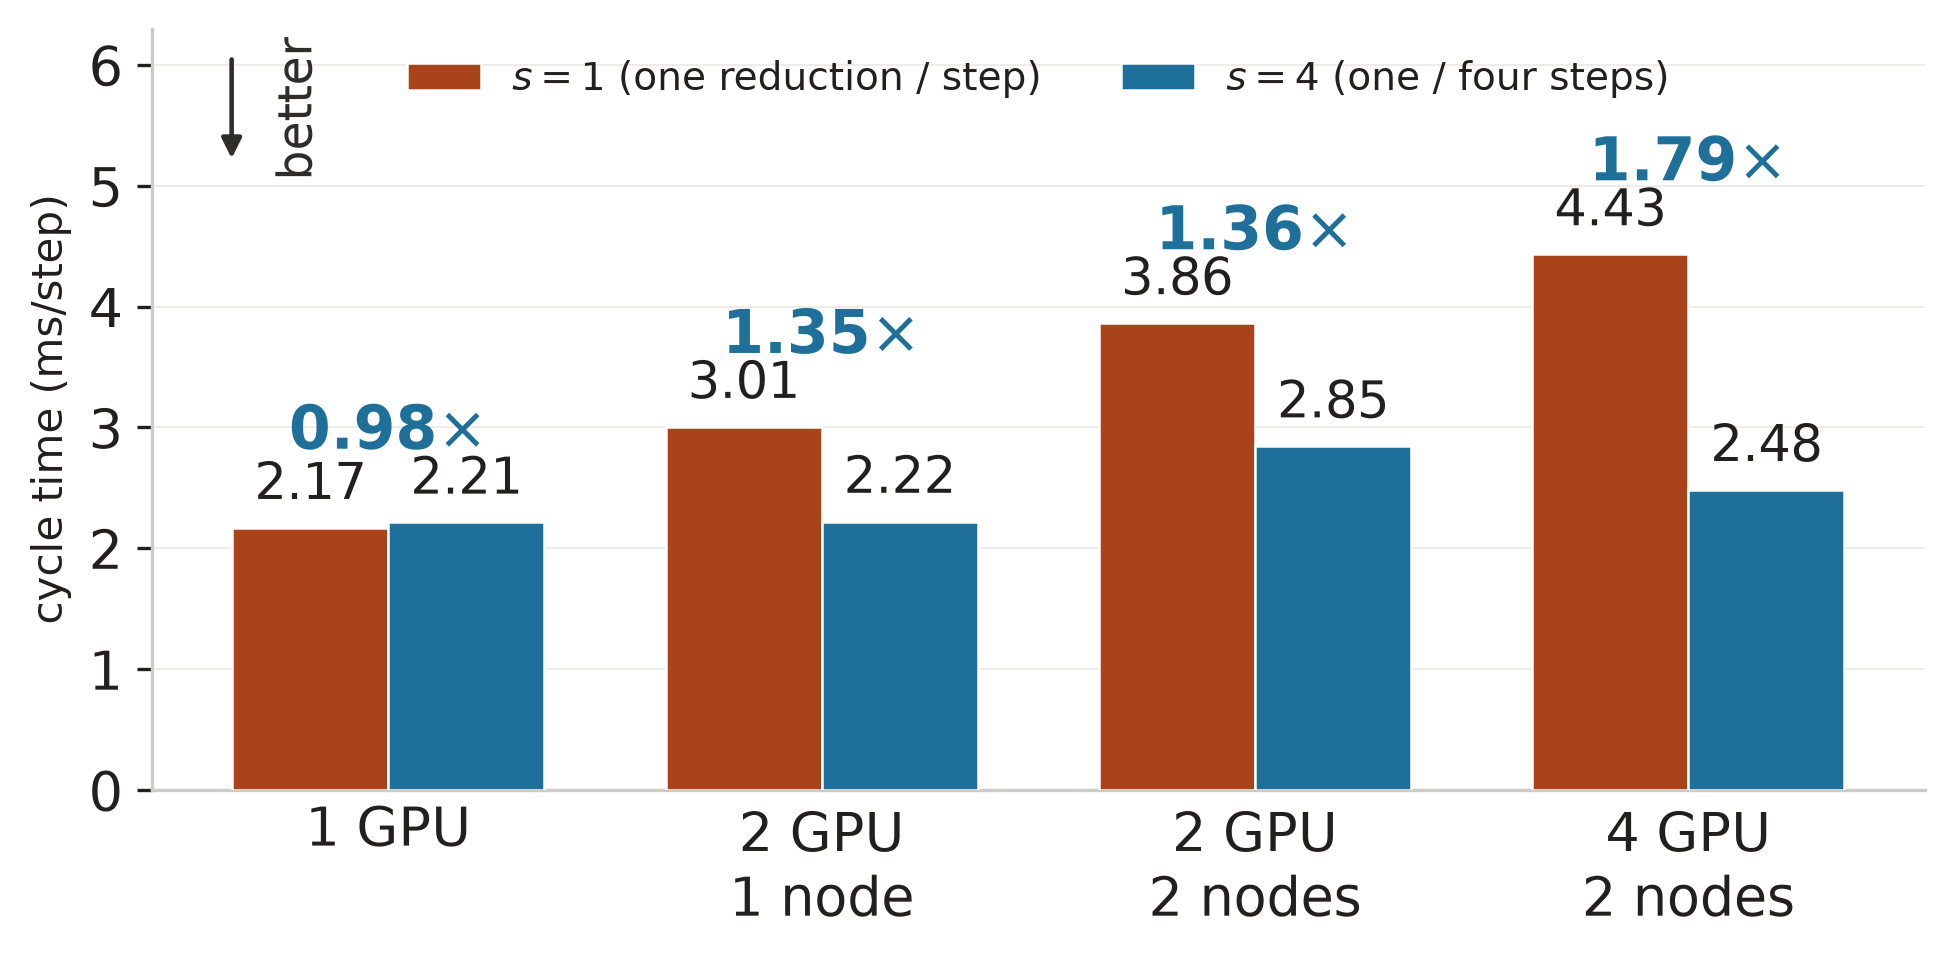
\includegraphics[width=0.92\linewidth]{ca_step_time_ladder.png}
  \end{figure}
  \vskip-1.2em
  \centerline{\scriptsize Basket, production grid $n{=}61$, 100 steps,
              \emph{exact-depth} halo: both widths do equal numerical work.}

  \vskip0.7em
  \begin{exampleblock}{}\footnotesize
    \centering
    Parity on one GPU, and \textbf{1.78--1.80$\times$} on four V100s across two
    nodes. Plane-streamed matrix powers add \textbf{1.21--1.32$\times$} on a
    single device.
  \end{exampleblock}

\end{frame}

% -----------------------------------------------------------
% SLIDE 11  |  The honest limit
% -----------------------------------------------------------
\begin{frame}[t]{The honest limit: CA helps, distribution still costs}
\small

  \vskip0.4em
  \begin{columns}[T]
    \column{0.49\textwidth}
    \vskip-0.8em
    \begin{figure}
      \centering
      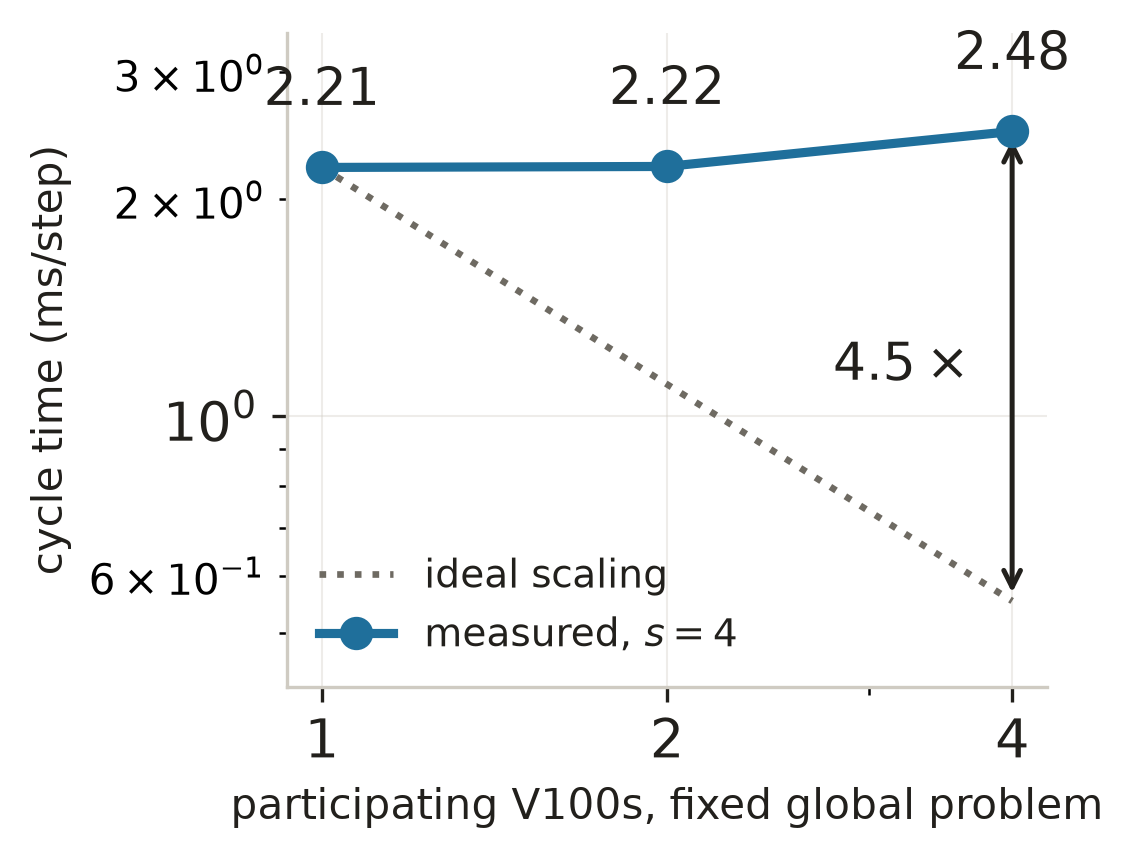
\includegraphics[width=\linewidth]{pres_honest_limit.png}
    \end{figure}
    \vskip-1.0em
    \centerline{\scriptsize \textbf{Strong:} fixed problem, more GPUs.}
    \centerline{\scriptsize $0.89\times$, about 22\% efficiency.}

    \column{0.49\textwidth}
    \vskip-0.8em
    \begin{figure}
      \centering
      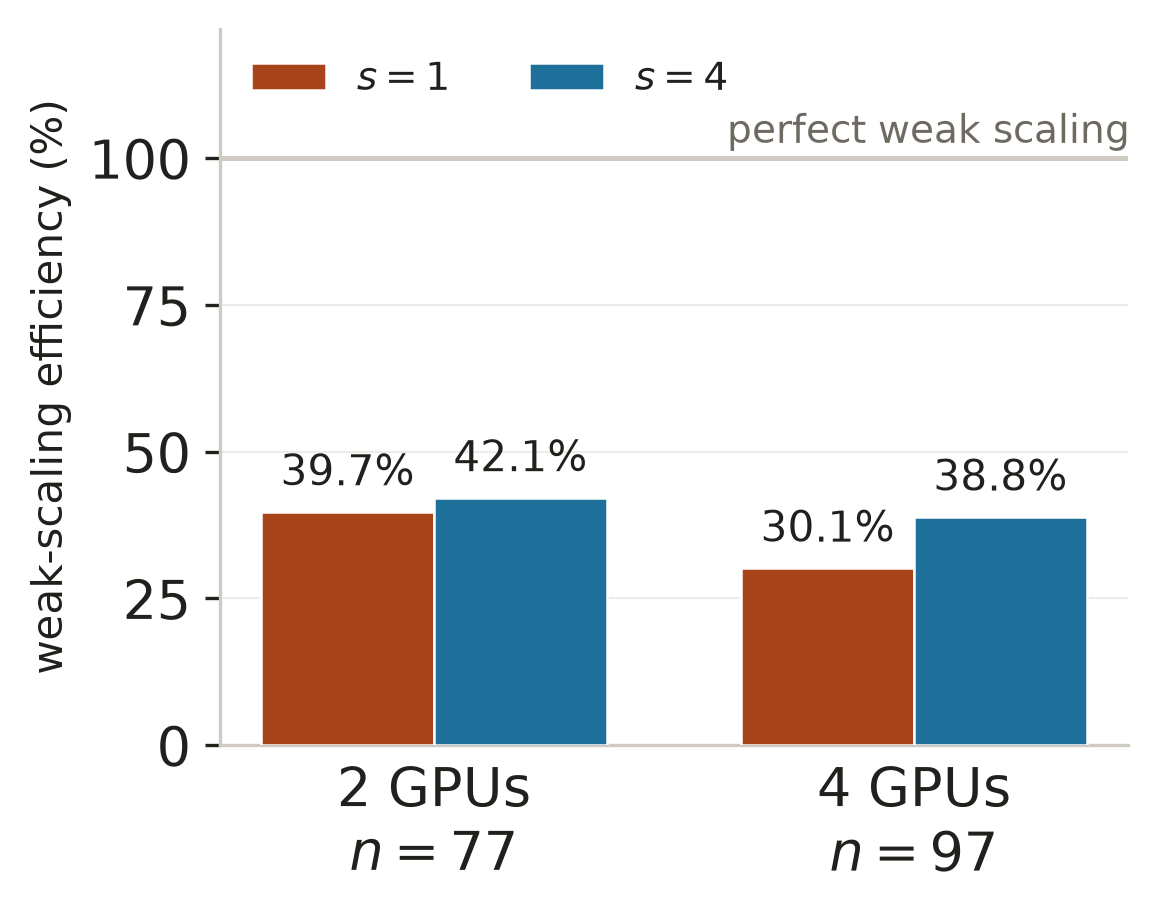
\includegraphics[width=\linewidth]{pres_weak_scaling.png}
    \end{figure}
    \vskip-1.0em
    \centerline{\scriptsize \textbf{Weak:} ${\approx}227{,}000$ rows per GPU held fixed.}
  \end{columns}

  \vskip0.7em
  \begin{alertblock}{}\footnotesize
    \centering
    At $n{=}61$ each of four slabs owns only ${\approx}57{,}000$ rows: too
    little to saturate a V100. Four GPUs earn their place \textbf{above
    $n=337$}, where the problem stops fitting on one card.
  \end{alertblock}

\end{frame}

% -----------------------------------------------------------
% SLIDE 12  |  Conclusions and future work
% -----------------------------------------------------------
\begin{frame}[t]{Conclusions and future work}
\small

  \begin{alertblock}{}
    \begin{center}
      Communication avoidance pays only when the \textbf{operator}, the
      \textbf{kernel} and the \textbf{machine} all line up.
    \end{center}
  \end{alertblock}

  \begin{columns}[T]
    \column{0.49\textwidth}
    \textbf{What the work establishes}
    \begin{itemize}\footnotesize
      \item Two a-priori coordinates that say \emph{which} mechanism is
            worth measuring, without timing the solver.
      \item One system where the corner is unreachable and one where more
            participants reach it, on the same definitions.
      \item A distributed CA integrator, \textbf{1.78--1.80$\times$} faster on
            four V100s, validated against independent references and
            \textbf{5.8--6.4$\times$} faster than smoothed ADI at equal
            declared accuracy.
    \end{itemize}

    \column{0.49\textwidth}
    \textbf{Future work}
    \begin{itemize}\footnotesize
      \item A \textbf{tile-aware $\Rv$} predicting read redundancy from tile
            dimensions, stencil radius and streamed height.
      \item \textbf{Mixed precision} recurrence with higher-precision Gram
            accumulation. Not free: a lower-precision basis worsens the very
            conditioning the guard tracks, so it must be gated on measured
            orthogonality.
      \item \textbf{H100-class devices and faster links}: does the crossover
            transfer beyond Synge?
    \end{itemize}
  \end{columns}

\end{frame}

% -----------------------------------------------------------
% Thank you
% -----------------------------------------------------------
{\setbeamertemplate{footline}{}
\begin{frame}[t]{Thank you}

  \vskip1.2em
  \begin{center}
    {\large This work stands on a great deal of help.}

    \vskip1.0em
    \begin{minipage}{0.86\textwidth}\small\centering
      My thanks to my supervisor, to the staff and students of the MSc in
      High-Performance Computing, to everyone who kept the clusters running,
      and to my family, for the teaching, the patience and the support that
      made it possible.
    \end{minipage}

    \vskip1.3em
    \begin{minipage}{0.80\textwidth}\centering
      \emph{``If I have seen further it is by standing on the shoulders of
      Giants.''}\\[0.3em]
      {\footnotesize Isaac Newton, letter to Robert Hooke, 5 February 1675}
    \end{minipage}

    \vskip1.3em
    {\Large Questions?}\\[0.8em]
    {\footnotesize
      Code: \href{https://github.com/kevinknights29/caksm}%
                 {\texttt{github.com/kevinknights29/caksm}}\\[0.25em]
      Thesis: \href{https://github.com/kevinknights29/caksm/blob/main/docs/thesis/main.pdf}%
                   {\texttt{.../caksm/docs/thesis/main.pdf}}}
  \end{center}

\end{frame}}

% ===========================================================================
\appendix
% ===========================================================================

{\setbeamertemplate{footline}{}
\begin{frame}[c]{}
  \vfill
  \begin{center}
    {\Large\bfseries\color{TCDBlue} Appendix}\\[0.8em]
    {\small Supporting detail, held in reserve.}
  \end{center}
  \vfill
\end{frame}}

% -----------------------------------------------------------
% A1  |  Financial numerical validation
% -----------------------------------------------------------
\begin{frame}[t]{Appendix: financial numerical validation}
\small

  Are the prices still right, and how does the solver compare with an
  established method? \textbf{KSM-EI} is the Krylov exponential integrator,
  \textbf{ADI-HV-S} the smoothed Hundsdorfer--Verwer ADI scheme.

  \vskip0.4em
  \begin{columns}[T]
    \column{0.52\textwidth}
    \centerline{\footnotesize\textbf{Equal declared accuracy, one thread, $n{=}61$}}
    \vskip-0.3em
    \begin{center}\scriptsize\setlength{\tabcolsep}{3pt}
    \begin{tabular}{@{}llrrr@{}}\toprule
      \textbf{Payoff} & \textbf{Method} & \textbf{Steps} & \textbf{Median (s)} & \\\midrule
      Basket  & ADI-HV-S & 50 & 3.090 & \\
      Basket  & KSM-EI   & 1  & 0.533 & \textbf{5.8$\times$} \\[0.2em]
      Rainbow & ADI-HV-S & 50 & 2.936 & \\
      Rainbow & KSM-EI   & 1  & 0.460 & \textbf{6.4$\times$} \\
      \bottomrule
    \end{tabular}
    \end{center}

    \column{0.46\textwidth}
    \centerline{\footnotesize\textbf{Where the price error actually is}}
    \vskip-0.3em
    \begin{center}\scriptsize\setlength{\tabcolsep}{2pt}
    \begin{tabular}{@{}lrr@{}}\toprule
      \textbf{Source of $\Delta$} & \textbf{Basket} & \textbf{Rainbow} \\\midrule
      reference       & $6.8\!\times\!10^{-6}$  & $<\!10^{-13}$ \\
      domain          & $1.0\!\times\!10^{-4}$  & $4.5\!\times\!10^{-6}$ \\
      \textbf{spatial}& $\mathbf{2.9\!\times\!10^{-3}}$ & $\mathbf{3.6\!\times\!10^{-2}}$ \\
      ADI temporal    & $2.2\!\times\!10^{-6}$  & $2.4\!\times\!10^{-5}$ \\
      KSM temporal    & $5.3\!\times\!10^{-15}$ & $3.6\!\times\!10^{-15}$ \\
      \bottomrule
    \end{tabular}
    \end{center}
  \end{columns}

  \vskip0.5em
  {\footnotesize
  Both solvers refine at second order against independent references.\\
  Basket $\Delta$ errors are 0.011--0.020\%. The ADI comparison is
  \textbf{Dang, Christara \& Jackson (2010)}, my last seminar paper.}

\end{frame}

% -----------------------------------------------------------
% A2  |  Numerical admissibility
% -----------------------------------------------------------
\begin{frame}[t]{Appendix: is the Krylov block numerically admissible?}
\small

  A monomial block $[\vect v,\mat A\vect v,\ldots,\mat A^{q-1}\vect v]$ loses
  conditioning fast, so CholeskyQR2 needs a guard.

  \vskip0.4em
  \begin{columns}[T]
    \column{0.50\textwidth}\footnotesize
    \textbf{What the implementation does.} It narrows the block whenever
    $\kappa_2(\mat Z) > u^{-1/2}\approx9.5\times10^{7}$.

    \smallskip
    \textbf{What theory covers.} The dimension-dependent sufficient condition
    $\delta = 8\kappa_2(\mat Z)\sqrt{Mqu+q(q+1)u}\le1$ limits $\kappa_2$ to
    ${\approx}1.25\times10^{4}$ at $M=226{,}984$, $q=4$. The measured block
    reaches $6.0\times10^{6}$, giving $\delta\approx482$: the theorem is
    \emph{inconclusive}, not violated.

    \smallskip
    Acceptance therefore rests on the guard, successful factorization,
    measured orthogonality, and referee agreement.

    \column{0.48\textwidth}
    \centerline{\footnotesize\textbf{Orthogonality loss, $n{=}61$, $m{=}8$, $q{=}4$}}
    \vskip0.2em
    \begin{center}\scriptsize\setlength{\tabcolsep}{4pt}
    \begin{tabular}{@{}lrr@{}}\toprule
      \textbf{Method} & $\|\mat I-\mat Q^{\mathsf T}\mat Q\|$ & \textbf{Time} \\\midrule
      CholeskyQR2 & $4.0\!\times\!10^{-14}$ & $1.00\times$ \\
      TSQR        & $3.5\!\times\!10^{-14}$ & $3.06\times$ \\
      Block GS, reorth. & $6.5\!\times\!10^{-14}$ & $1.24\times$ \\
      \bottomrule
    \end{tabular}
    \end{center}
    \vskip0.5em
    \centerline{\footnotesize\textbf{Width admitted by the guard}}
    \vskip0.2em
    \begin{center}\scriptsize\setlength{\tabcolsep}{6pt}
    \begin{tabular}{@{}lcc@{}}\toprule
      \textbf{Basis} & $n{=}31$ & $n{=}61$ \\\midrule
      Monomial  & \textbf{4} & \textbf{4} \\
      Newton (Leja) & 3 & 3 \\
      Chebyshev & 4 & 3 \\
      \bottomrule
    \end{tabular}
    \end{center}
  \end{columns}

\end{frame}

% -----------------------------------------------------------
% A3  |  The cache-aware roofline
% -----------------------------------------------------------
\begin{frame}[t]{Appendix: the cache-aware roofline on puffin}
\small

  \vskip-0.3em
  \begin{columns}[c]
    \column{0.52\textwidth}
    \begin{figure}
      \centering
      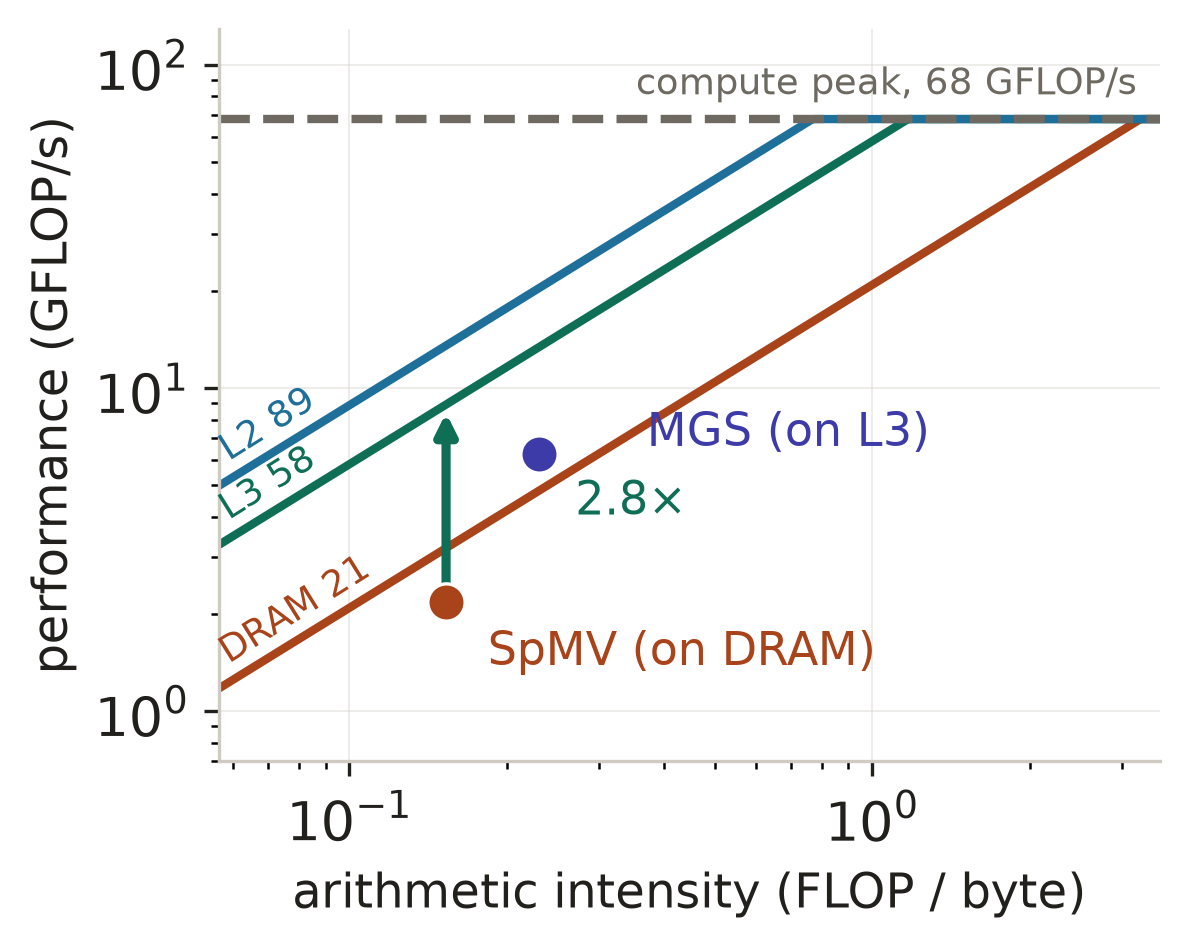
\includegraphics[width=\linewidth]{pres_cache_roofline.png}
    \end{figure}
    \vskip-1.0em
    \centerline{\scriptsize One core, $n{=}61$.}

    \column{0.45\textwidth}
    \begin{center}\footnotesize\setlength{\tabcolsep}{4pt}
    \begin{tabular}{@{}lcc@{}}\toprule
      \textbf{Kernel} & $AI$ & \textbf{Tier} \\\midrule
      SpMV                   & 0.15 & DRAM \\
      MGS                    & 0.23 & L3 \\
      dense $\exp(\mat H_m)$ & 1.76 & L2 \\\bottomrule
    \end{tabular}
    \end{center}
    \vskip-0.2em
    \centerline{\scriptsize arithmetic intensity, FLOP per byte}
  \end{columns}

  \vskip1.2em
  \centerline{$\displaystyle
    \text{gain}=\frac{\min(BW_{\text{fast}}\!\cdot\!AI,\ \text{peak})}
                     {\min(BW_{\text{slow}}\!\cdot\!AI,\ \text{peak})}
    = \frac{58.2}{20.9} = \mathbf{2.8\times}
    \quad\text{at } AI=0.15 .$}

\end{frame}

% -----------------------------------------------------------
% A4  |  Where a GPU differs from a CPU
% -----------------------------------------------------------
\begin{frame}[t]{Appendix: where a GPU differs from a CPU}
\small

  \vskip-0.2em
  \begin{center}
  \scalebox{0.80}{%
  \begin{tikzpicture}[
    core/.style={draw=TCD-Blue,fill=TCDBlue,text=white,font=\tiny,
                 minimum width=0.42cm,minimum height=0.32cm,inner sep=1pt},
    sm/.style={draw=TCD-Blue,fill=TCDBlue,text=white,font=\tiny,
               minimum width=0.34cm,minimum height=0.32cm,inner sep=1pt},
    cache/.style={draw=TCD-Grey-ii,fill=TCD-Grey-iii,font=\scriptsize,
                  text=TCD-Grey,minimum height=0.38cm},
    ccx/.style={draw=TCD-Grey-ii,rounded corners=2pt,inner sep=3pt},
    lbl/.style={font=\scriptsize,text=TCD-Grey}]

    \node[font=\small\bfseries,text=TCD-Grey] at (2.20,2.62)
      {\textbf{CPU} --- puffin, Threadripper 3960X};
    \foreach \k in {0,1,2}{
      \begin{scope}[xshift=\k*1.70cm]
        \foreach \i in {0,1,2}{\node[core] at (\i*0.46,1.85) {};}
        \node[cache,minimum width=1.36cm] at (0.46,1.35) {16\,MiB L3};
        \node[ccx,fit={(-0.26,1.14) (1.18,2.05)}] {};
      \end{scope}}
    \node[lbl] at (5.35,1.60) {$\cdots\times 8$};

    \node[font=\small\bfseries,text=TCD-Grey] at (9.30,2.62)
      {\textbf{GPU} --- synge, Tesla V100};
    \foreach \i in {0,...,7}{\node[sm] at (6.55+\i*0.66,1.85) {};}
    \node[lbl] at (12.02,1.85) {$\cdots\times 80$};
    \node[cache,minimum width=6.20cm] at (9.30,1.35) {one shared 6\,MB L2};
    \node[ccx,fit={(6.15,1.14) (12.55,2.05)}] {};
  \end{tikzpicture}}
  \end{center}

  \vskip0.5em
  \begin{columns}[T]
    \column{0.48\textwidth}\footnotesize
    \textbf{CPU}
    \begin{itemize}
      \item Cache \textbf{grows with the team}: each engaged core complex
            brings its own L3 slice.
      \item $\Rv$ scales with the engaged core count $P$, so the two axes are
            coupled and $\Rv\Rh$ is roughly $P$-independent.
      \item Reductions cross \textbf{2} levels.
    \end{itemize}

    \column{0.48\textwidth}\footnotesize
    \textbf{GPU}
    \begin{itemize}
      \item Cache is \textbf{fixed}: engaging more SMs adds none.
      \item $\Rv$ stops depending on how many SMs are engaged, so
            \textbf{grid size alone moves it}.
      \item Reductions cross \textbf{5} levels, one of them a kernel launch.
            Coalescing also makes the access pattern far more sensitive.
    \end{itemize}
  \end{columns}

\end{frame}

% -----------------------------------------------------------
% A5  |  The reduction ladder
% -----------------------------------------------------------
\begin{frame}[t]{Appendix: the reduction ladder and $\tredstar$}
\small

  \vskip-0.4em
  \begin{center}
  \scalebox{0.66}{%
  \begin{tikzpicture}[
    gpu/.style={draw=TCD-Blue,fill=TCDBlue,text=white,
                font=\small\bfseries,minimum width=1.6cm,minimum height=0.55cm},
    nodebox/.style={draw=TCD-Grey-ii,rounded corners=2pt,inner sep=7pt},
    lbl/.style={font=\footnotesize,text=TCD-Grey}]
    \node[gpu] (a1) at (0,0)   {V100};
    \node[gpu] (a2) at (2.2,0) {V100};
    \draw[TCDBlue,very thick] (a1) -- (a2);
    \node[nodebox,fit=(a1)(a2)] (n1) {};
    \node[lbl,anchor=north] at ([yshift=-2pt]n1.south) {PCIe + cross-socket, $11.46\,\mu$s};
    \node[lbl,anchor=south west] at ([yshift=-1pt]n1.north west) {\texttt{synge-n01}};

    \node[gpu] (b1) at (7.6,0)  {V100};
    \node[gpu] (b2) at (9.8,0)  {V100};
    \draw[TCDBlue,very thick] (b1) -- (b2);
    \node[nodebox,fit=(b1)(b2)] (n2) {};
    \node[lbl,anchor=north] at ([yshift=-2pt]n2.south) {two V100s per node};
    \node[lbl,anchor=south west] at ([yshift=-1pt]n2.north west) {\texttt{synge-n02}};

    \node[draw=TCD-Grey-ii,fill=TCD-Grey-iv,minimum height=1.1cm,
          font=\footnotesize,align=center] (fab) at (4.9,0)
          {Omni-Path fabric\\$22.09\,\mu$s};
    \draw[TCD-Grey,thick] (n1.east) -- (fab.west);
    \draw[TCD-Grey,thick] (fab.east) -- (n2.west);
  \end{tikzpicture}}
  \end{center}

  \vskip0.3em
  \centerline{$\displaystyle
    \Rv\Rh = g(m)\,R(m)\,\Lambda ,
    \qquad
    \Lambda=\frac{\tred\cdot BW}{C}
    \qquad\Longrightarrow\qquad
    \tredstar = 0.69\,\mu\text{s}$}
  \vskip0.2em
  \centerline{\footnotesize priced at the production point $n{=}61$, $m{=}17$.}

  \vskip0.4em
  \begin{center}\footnotesize\setlength{\tabcolsep}{10pt}
  \begin{tabular}{@{}lrc@{}}\toprule
    \textbf{Reduction rung} & $\tred$ \textbf{($\mu$s)} & \textbf{Corner} \\\midrule
    warp shuffle       & 0.42  & closed \\
    thread block       & 0.79  & \textbf{open} \\
    grid, 2nd launch   & 5.54  & \textbf{open} \\
    device, PCIe       & 11.46 & \textbf{open} \\
    node, fabric       & 22.09 & \textbf{open} \\
    \bottomrule
  \end{tabular}
  \end{center}

  \vskip0.3em
  \centerline{\scriptsize Puffin, for comparison: $t_{\text{intra}}=120.8$\,ns,
              $t_{\text{cross}}=652.8$\,ns, $L^{\star}=2.20$, $R^2=0.98$.}

\end{frame}

% -----------------------------------------------------------
% A6  |  Memory access is the CPU's binding constraint
% -----------------------------------------------------------
\begin{frame}[t]{Appendix: on the CPU, memory access is the binding constraint}
\small

  \begin{columns}[T]
    \column{0.50\textwidth}
    \vskip-1.2em
    \begin{figure}
      \centering
      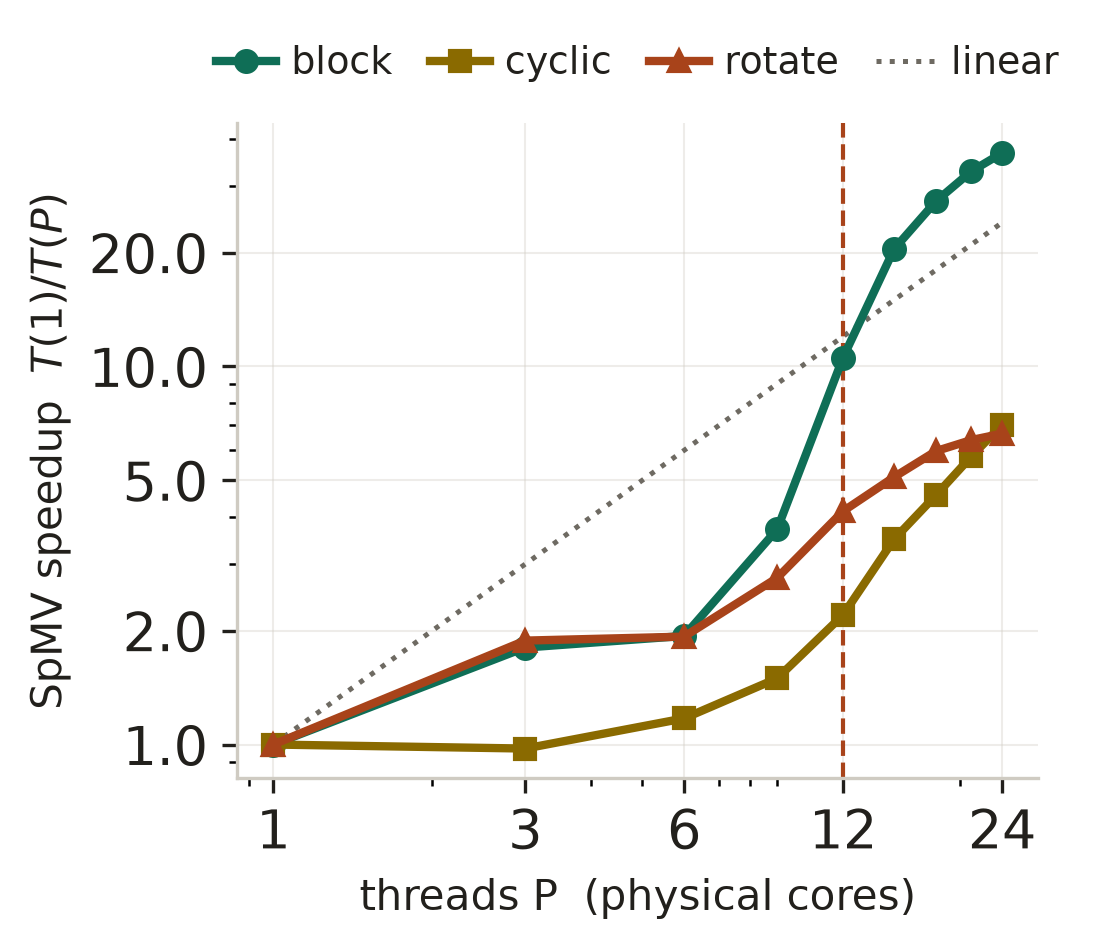
\includegraphics[width=\linewidth]{pres_scaling_locality.png}
    \end{figure}
    \vskip-1.1em
    \centerline{\scriptsize Same operator and byte count;}
    \centerline{\scriptsize only the row-to-core map changes.}

    \column{0.48\textwidth}
    \vskip0.2em
    \begin{center}\scriptsize\setlength{\tabcolsep}{2pt}
    \begin{tabular}{@{}llr@{}}\toprule
      \textbf{\texttt{schedule}} & \textbf{Rows per core} & \textbf{Speedup} \\\midrule
      \texttt{block}  & contiguous band        & \textbf{36.7$\times$} \\
      \texttt{cyclic} & same bytes, dealt out  & 7.0$\times$ \\
      \texttt{rotate} & contiguous, reshuffled & 6.6$\times$ \\
      \bottomrule
    \end{tabular}
    \end{center}
    \vskip-0.2em
    \centerline{\scriptsize the OpenMP \texttt{schedule} clause}

    \vskip1.0em
    \footnotesize
    At the knee the implied 176\,GB/s exceeds puffin's ${\sim}95$\,GB/s DRAM
    roof, so it comes from L3.
    \textbf{Contiguity, not volume, keeps a slice resident.}
  \end{columns}

  \vskip0.4em
  \begin{alertblock}{}\footnotesize
    On one NUMA node no reduction costs more than a core-complex hop, so
    synchronization is never dominant: the lever here is \textbf{access order},
    not communication avoidance.
  \end{alertblock}

\end{frame}

% -----------------------------------------------------------
% A7  |  Plane streaming
% -----------------------------------------------------------
\begin{frame}[t]{Appendix: the kernel schedule, not the tile}
\small

  \vskip-0.3em
  \begin{figure}
    \centering
    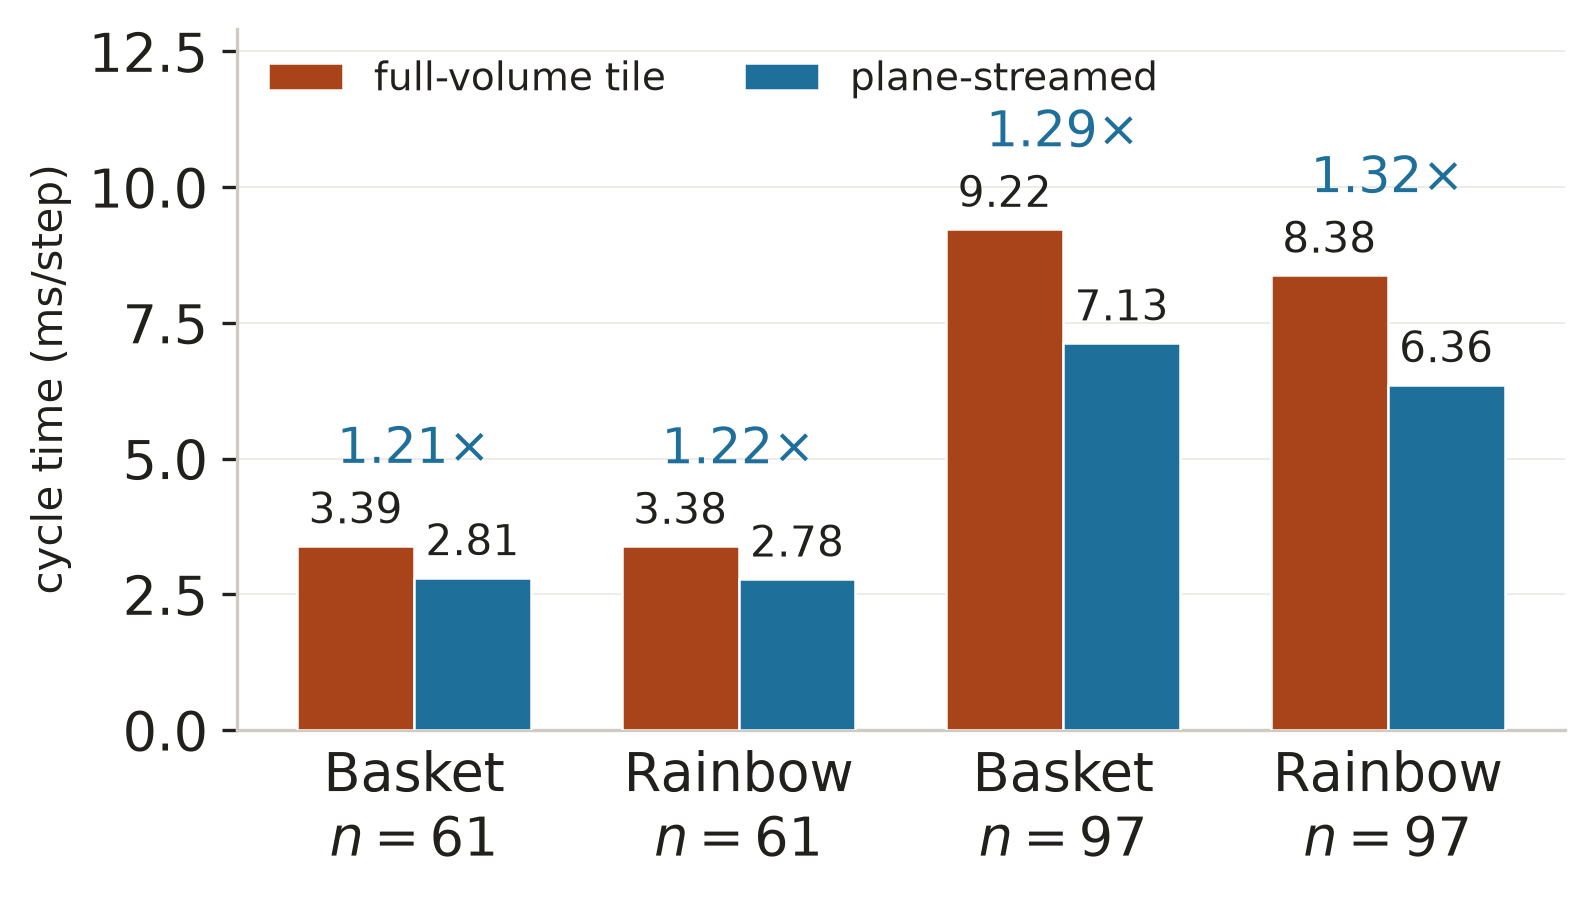
\includegraphics[width=0.55\linewidth]{pres_plane_streaming.png}
  \end{figure}
  \vskip-1.1em
  \centerline{\scriptsize One V100. The $x$--$y$ tile is fixed at
              $16\times8$; only the order in which a block walks $z$ changes.}

  \vskip0.7em
  \centerline{\footnotesize\textbf{Nsight counters, full-volume $\to$ plane-streamed}}
  \vskip0.3em
  \begin{center}\footnotesize\setlength{\tabcolsep}{9pt}
  \begin{tabular}{@{}lcc@{}}\toprule
    & $n{=}61$ & $n{=}97$ \\\midrule
    thread blocks launched & 2{,}048 $\to$ 256 & 8{,}125 $\to$ 637 \\
    executed instructions  & $2.9\times$ fewer & $3.4\times$ fewer \\
    global-load sectors    & \multicolumn{2}{c}{$2.6$--$4.2\times$ fewer} \\
    \bottomrule
  \end{tabular}
  \end{center}
  \vskip-0.3em
  \centerline{\scriptsize Each plane is fetched from global memory \emph{once}
              and reused down the segment.}

  \vskip0.4em
  \centerline{\footnotesize\textbf{This does not replace $s$-step; it composes with it.}}

\end{frame}

% -----------------------------------------------------------
% A8  |  The memory footprint
% -----------------------------------------------------------
\begin{frame}[t]{Appendix: when does the problem stop fitting on one card?}
\small

  \vskip0.8em
  \begin{center}\footnotesize\setlength{\tabcolsep}{12pt}
  \begin{tabular}{@{}lrr@{}}\toprule
    \textbf{FP64 footprint} & $n{=}61$ & $n{=}337$ \\\midrule
    unknowns $N$                    & $2.27\times10^{5}$ & $3.83\times10^{7}$ \\
    one state vector (GB)           & $1.8\times10^{-3}$ & $3.1\times10^{-1}$ \\
    Krylov basis, $m{=}39$ (GB)     & $7.1\times10^{-2}$ & $1.19\times10^{1}$ \\
    share of a 16\,GB V100          & 0.4\%              & \textbf{75\%} \\
    \bottomrule
  \end{tabular}
  \end{center}

  \vskip1.0em
  \begin{exampleblock}{}\footnotesize
    \centering
    $n=337$ is the largest odd grid common to every topology, payoff and width
    after a 10\% memory reserve. The binding arm is the \emph{one-GPU},
    $s{=}4$ case, which is exactly why four GPUs start to earn their place
    above it.
  \end{exampleblock}

  \vskip0.6em
  {\footnotesize
  At that grid the predeclared numerical gate converges with maximum $m=32$ and
  residual $9.85\times10^{-9}$, but the boundary-state gate fails at
  $6.40\times10^{-5}$. Rescaling the augmentation by $\eta=2^{-36}$ repairs it
  to $4.41\times10^{-13}$; the original stop remains the reported result.}

\end{frame}

\end{document}
